% $Header: /cvsroot/latex-beamer/latex-beamer/examples/beamerexample3.tex,v 1.8 2004/10/07 20:53:07 tantau Exp $

\documentclass{beamer}

% \usepackage{bbding}
%\usepackage[utf8]{inputenc}
\usepackage[latin1]{inputenc}
\usepackage{graphicx}
\usepackage{epsfig}
%\usepackage{colortbl}
\usepackage{amsfonts}
\usepackage{verbatim}
\font\sevenex=cmex7
\scriptfont3=\sevenex \scriptscriptfont3=\sevenex
% \logo{\includegraphics[width=1.58cm]{../../../figures/code_devel/lbnl_logo.eps}}
% \useoutertheme{infolines}
% \setbeamertemplate{footline}{\raisebox{-2ex}{\pgfuseimage{institut-logo}}
%   \usebeamerfont{date in head/foot}\insertshortdate{}\hfill
%   \usebeamertemplate{navigation symbols}\hfill
%   \insertframenumber{}/\inserttotalframenumber}



\mode<presentation>
{
%    \usetheme{PaloAlto}
   \usetheme{Warsaw}

   \setbeamercovered{transparent}
} 	

% \setbeamercovered{transparent}

\title[LCLS-II LLRF Review]{LCLS-II LLRF Review: Simulations}

% \author[ATG@LBNL]{C. Serrano}

\institute[SLAC/LBNL]{SLAC/LBNL}
% \date[LBNL]{LBNL, Berkeley, Sept 19, 2013}


%-----------document--------------

\begin{document}

\frame{\titlepage}


\part{Contents}

\section{Integrated simulations: Tracking+LLRF+BBF}

\frame{
	\frametitle[]{NGLS Feedback}
	\begin{figure}
	  \centering
	  \includegraphics[scale=0.35]{figures/ngls_feedback.pdf}
	\end{figure}
}

\frame{
	\frametitle[]{Software data flow}
	\begin{figure}
	  \centering
	  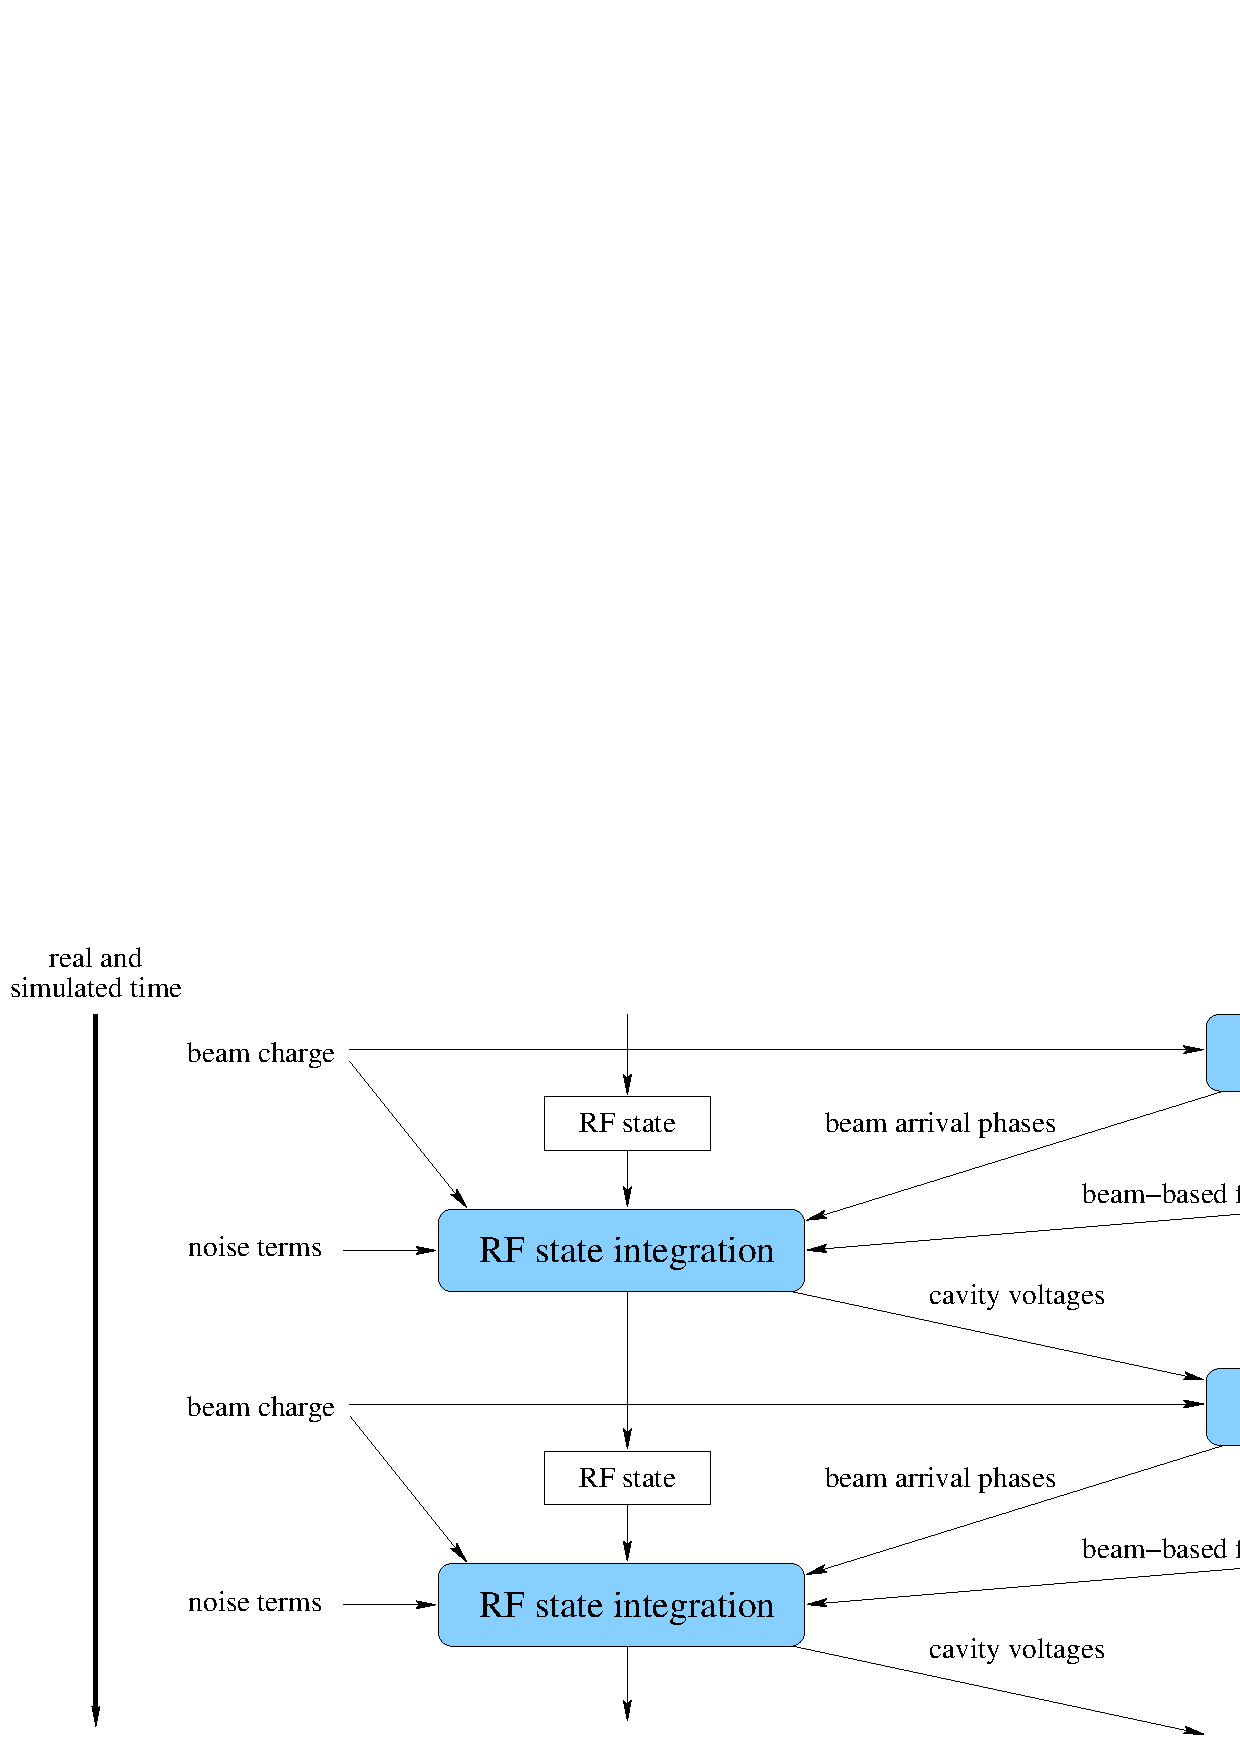
\includegraphics[scale=0.30]{figures/model_do2.pdf}
	\end{figure}
}

\frame{
	\frametitle[]{Model capabilities}
	\begin{block}{Particle tracking + LLRF/BBF integrated models}
		\begin{center}
		Particles are tracked down the LINAC, properties measured and fed-back using accurate LLRF and BBF models.
		\end{center}
	\end{block}
	\begin{block}{Noise Sources and processing}
		\begin{center}
		Abilty to inject noise at any location of the machine and quantify how it propagates thoughout the LINAC.
		\end{center}
	\end{block}
	\begin{block}{Transfer functions}
		\begin{center}
		Transfer functions between any two points of the machine are calculated to evaluate effect of different noise sources on machine's performance/stability parameters. 
		\end{center}
	\end{block}
}

\frame{
  \frametitle[]{Requirements}
    \begin{itemize}
      \item Accurate models.
      \item Performance optimizations:
      \begin{itemize}
       \item Computation speed,
       \item Memory usage.
      \end{itemize}
    \item Modularity:
      \begin{itemize}
       \item Unit tests,
       \item Ease of re-implementation of different building blocks,
      \end{itemize}
      \item Configuration:
      \begin{itemize}
       \item Configuration file management: Storage and tracking,
       \item Flexibility to implement different Linac configurations easily.
      \end{itemize}
      \item High-level software:
      \begin{itemize}
       \item Back-end with API/hooks to interface with high-level software,
       \item Web-based user-friendly front-end.
      \end{itemize}

    \end{itemize}

}

\frame{
  \frametitle[]{Architecture}
    \begin{columns}[t]
    \begin{column}[T]{0.6\textwidth}
      \begin{enumerate}
        \item User edits files in browser front-end
        \item Client sends JSON files to Server
        \item Server executes simulation Python
        \item Python configures and calls wrapped C code
        \item Output files post-processed in Python
        \item Server sends data and plots to client
        \item Browser software renders plots
        \end{enumerate}
    \end{column}
    \begin{column}[T]{0.5\hsize}
      \includegraphics[height=0.8\textheight]{figures/architecture2}
    \end{column}
  \end{columns}
}

\frame{
  \frametitle[]{Simulation Code Structure}
  \begin{columns}[t]
    \begin{column}[T]{0.45\textwidth}
      Simulation split into C and Python:
      \begin{itemize}
      \item Python top level for reading configuration files and post-processing.
      \item C code implementing computationally intensive inner loop.
      \item Swig automatically wraps C functions and data structures.
        \begin{itemize}
        \item Accessing C arrays from Python slightly clumsy.
        \end{itemize}
      \end{itemize}
    \end{column}
    \begin{column}[T]{0.55\hsize}
      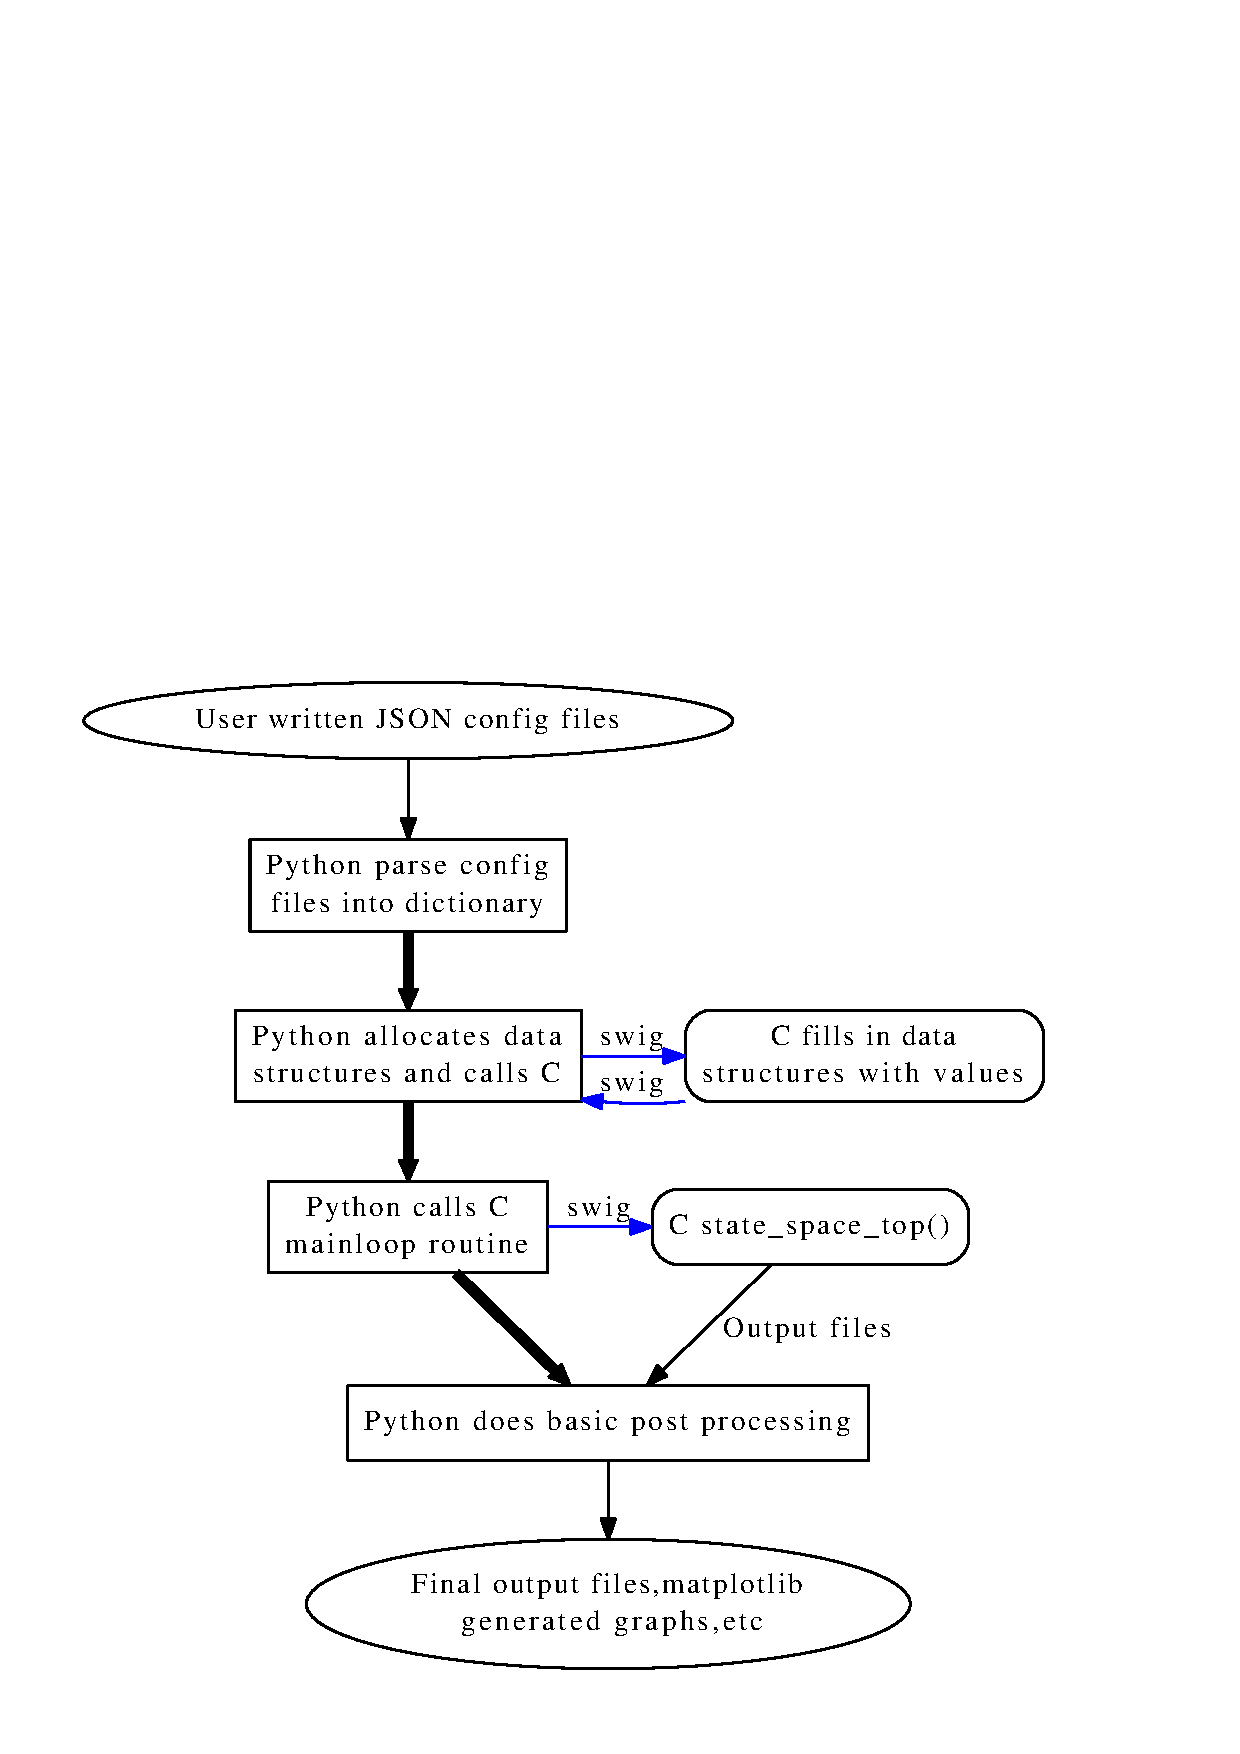
\includegraphics[height=0.9\textheight]{figures/shallowoutline}
    \end{column}
  \end{columns}
}

\frame{
  \frametitle[]{Improvements of the new generation Python/C code}
  \begin{itemize}
  \item Speed: 30 seconds to compute 1.2 million full simulation steps. 
  \item Memory: Configurable set of timeseries data stored in memory for analysis.
  \item Flexibility: Linac structure can be rearranged and reconfigured easily in configurations (NGLS, FLASH, LCLS-II can all be simulated).
  \item Documented and commented code.
  \item Verification via unit tests.
  \item Python top level is very powerful for development and enables easy interfaces with other codes.
  \end{itemize}
}

\frame{
  \frametitle[]{Example Parameter Search}
  \begin{itemize}
   \item Python's multiprocessing library makes multi core batching easy.
   \item Possibity of running simulations in parallel sweeping certain conditions (for example feedback settings) and optimizing a parameter search numerically.
  \end{itemize}

  \centerline{
  \includegraphics[height=0.6\textheight]{figures/gen_alg.pdf}
  }
}

\frame{
  \frametitle[]{User interface}
    \begin{itemize}
     \item ATG is migrating to JavaScript-based front ends,
     \item Server/client architecture where server generates JSON files and runs models,
     \item No need to install software or dependencies locally to run models and visualize results: Models can run in a powerful server to serve several clients,
     \item User-friendly interface enabling focus on science and hiding implementation details from the user.
    \end{itemize}
}

\frame{
  \frametitle{Simulaton screenshot}
    \begin{figure}
	  \centering
	  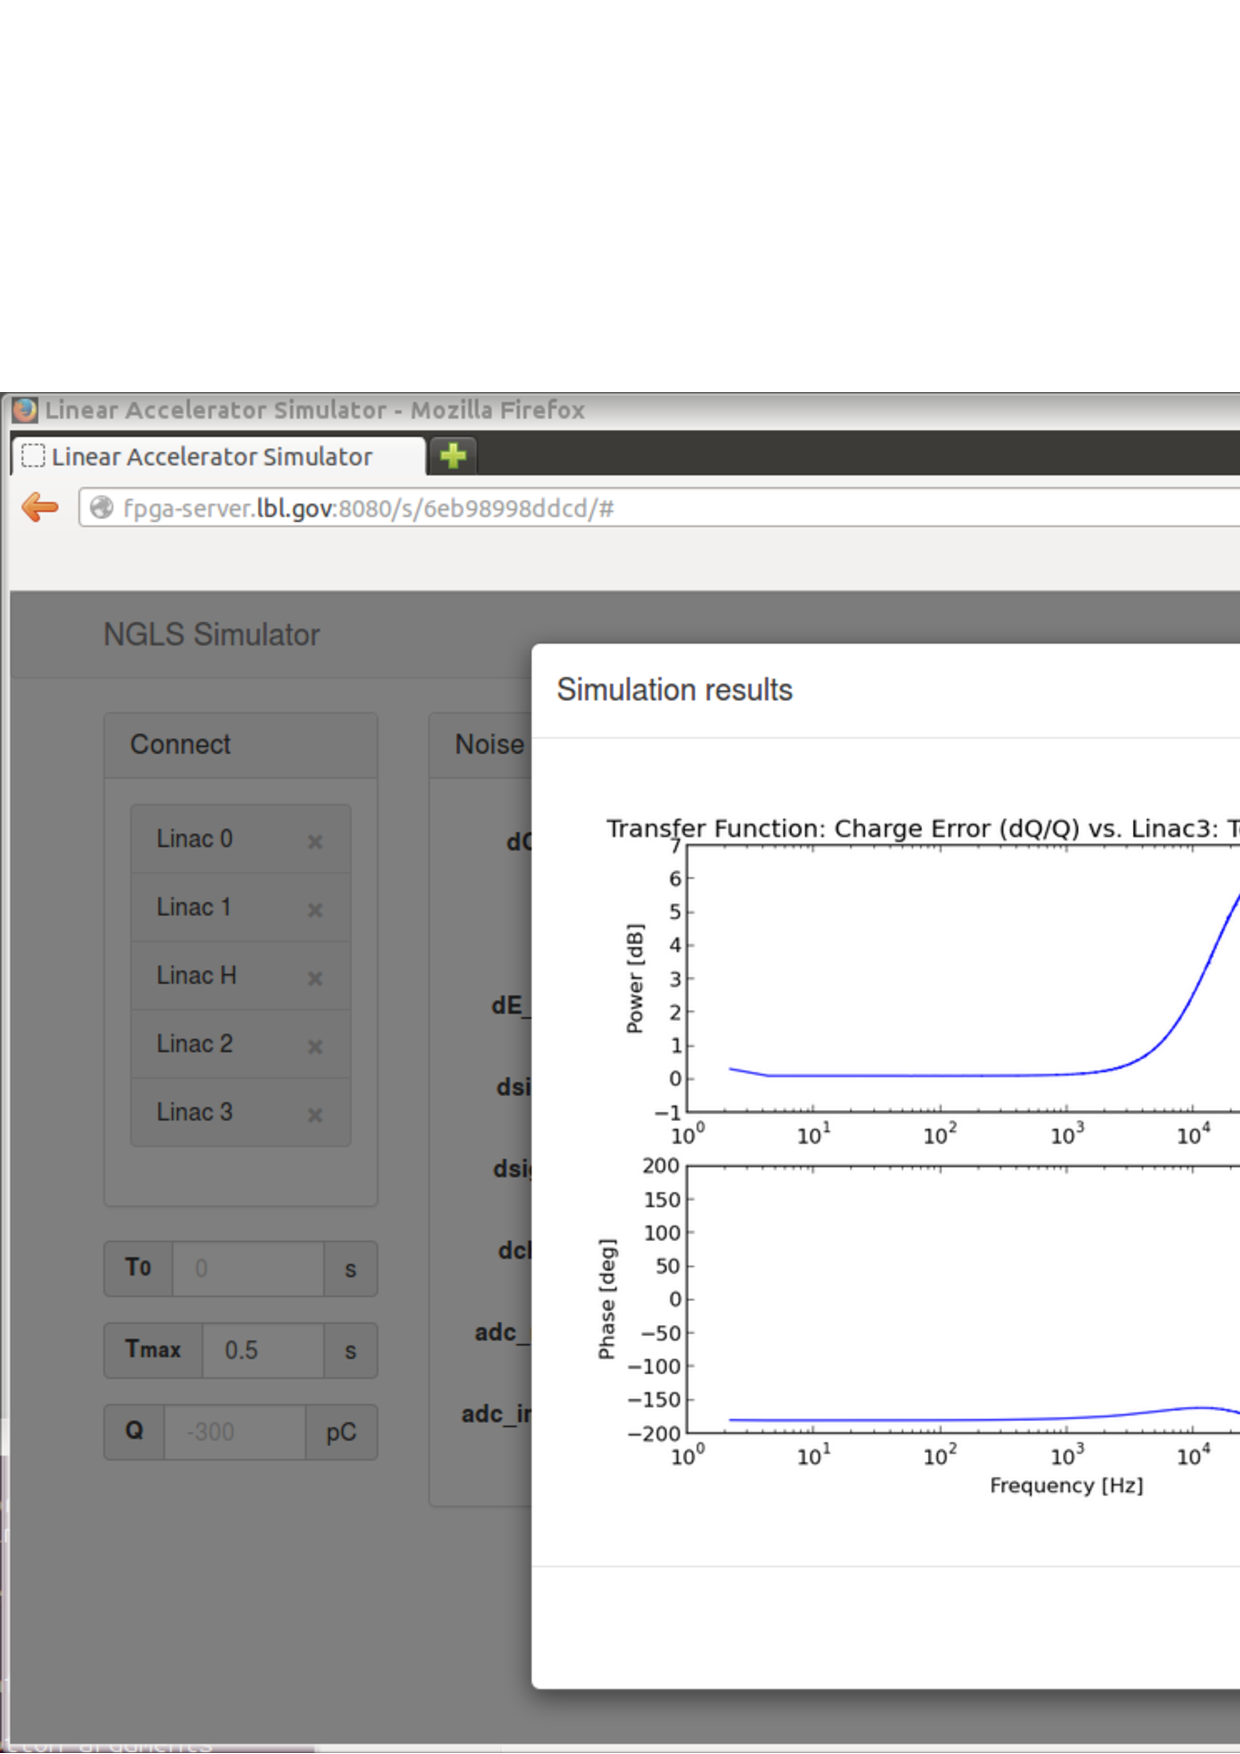
\includegraphics[scale=0.3]{figures/simulator_screenshot.pdf}
  \end{figure}
    
}

\section{FPGA design: HW/SW co-simulation}

\frame{
  \frametitle[]{HW/SW co-simulation}
      \begin{itemize}
        \item Three simulation modes:
	\begin{itemize}
	 \item Standalone SW simulation: Everything (including FPGA controller) in C/Python, etc.
	 \item Mixed HDL and Software: FPGA controller in synthesizable Verilog interacting with SW plant models.
	 \item Standalone HDL simulation: Run closed-loop simulations inside the FPGA to exercise FPGA-host link and user interfaces.
	\end{itemize}
	\item Cycle accurate synthesizable Verilog simulations: what is simulated is exactly what goes in the FPGA.
	\item After simulation cycle is completed:
	\begin{itemize}
	 \item Algorithmic issues have been solved in the comfortable environment of a computer.
	 \item Digital design/performance issues have been dealt with in the comfortable environment of a computer.
	 \item Communication and user interface issues have been dealt with on the bench.
	\end{itemize}

      \end{itemize}
}	
 

\frame{
	\frametitle[]{FPGA design: HW/SW co-simulation (Mixed HDL and Software)}
	\begin{figure}
	  \centering
	  \includegraphics[scale=0.18]{figures/LLRF_simulation_blocks.pdf}
	\end{figure}
}

\section{Cavity mechanical resonances}

\frame{
  \frametitle[]{Cavity mechanical resonances}
      \begin{itemize}
	 \item Currently single cavity with three mechanical modes.
	 \item Python/C/JSON architecture, which can easily:
	 \begin{itemize}
	  \item Scale to many cavities + complex coupling schemes,
	  \item Include computation of many cavity modes from random generators or measurements,
	  \item Automatically generate configuration files and parse them within Python to fill in C backend data structures,
	  \item Integrate with the rest of the simulation code (Tracking+BBF+LLRF).
	 \end{itemize}
    \end{itemize}
}
 
\frame{
	\frametitle[]{Cavity mechanical resonances}
  \begin{itemize}
   \item Single cavity falling off the cliff,
   \item System moves violently at both fall time and recovery time, enough that it could easily trigger nearby cavities to crash.
  \end{itemize}
	\begin{figure}
	  \centering
	  \includegraphics[scale=0.15]{figures/mech_modes.pdf}
	\end{figure}
}

\frame{
  \frametitle[]{Cavity mechanical resonances (timing)}
	  \begin{itemize}
	   \item t=0.0 s: Ramp up power according to sqrt(t) with 200 ms rise time. Piezo operates with I feedback to hold phase angle at 11 degrees,
	   \item t=0.2 s: Start passive decay towards equilibrium gradient,
	   \item t=0.5 s: Turn off piezo loop, artificially start drifting RF phase towards the cliff,
	   \item t$\approx$1.2 s: Cliff happens,
	   \item t=1.5 s: End artificial RF phase drift,
	   \item t=2.0 s: Turn piezo loop back on,
	  \end{itemize}
}



\end{document} 
